\documentclass[technicalreport]{ieicej}
\usepackage[dvipdfmx]{graphicx}
\usepackage[T1]{fontenc}
\usepackage{lmodern}
\usepackage{textcomp}
\usepackage{latexsym}
\usepackage{amsmath}
\usepackage{cite}
\usepackage{tikz}
\usepackage{geometry}
\usepackage{url}


\renewcommand{\figurename}{Fig.} % name the picture Fig.num
\renewcommand{\tablename}{Table } % name the table Table num
\renewcommand{\refname}{REFERENCE} % insert reference 

%调整文件显示位置和纸张
\geometry{
	a4paper,
	total={170mm,257mm},
	left=20mm,
	top=20mm,
}

\hoffset=-5mm
\voffset=-5mm

\def\IEICEJcls{\texttt{ieicej.cls}}
\def\IEICEJver{3.0}
\newcommand{\AmSLaTeX}{%
$\mathcal A$\lower.4ex\hbox{$\!\mathcal M\!$}$\mathcal S$-\LaTeX}
\def\BibTeX{{\rmfamily B\kern-.05em{\scshape i\kern-.025em b}\kern-.08em
T\kern-.1667em\lower.7ex\hbox{E}\kern-.125em X}}

\jtitle{M1課題レポート 第1回目}
\jsubtitle{}
\etitle{Technical Report for M1 Labwork 1-st}
\esubtitle{}
\authorlist{ % author name list
\authorentry[liuyuchen@radio.ict.e.titech.ac.jp]{りゅう ゆしん}{Yuchen Liu}{Titech}
}

\affiliate[Titech]{東京工業大学 〒152-8550 東京都目黒区大岡山2-12-1}
{Tokyo Institute of Technology,~~2-12-1, O-okayama, Meguro-ku, Tokyo, 152-8550 Japan}


\begin{document}
\maketitle

\section{Introduction}
This is the first C seminar which is \cite{wiki:Additive_white_Gaussian_noise}

\section{QPSK and MLE Background}

\begin{table}[tbp]
	\begin{center}
	\caption{ACRONYMS AND FULL MEANING}
	\begin{tabular}{|l|l|}
	\hline
	\textbf{Acronyms} & \textbf{Full Form} \\
	\hline
	 MLE & Maximum Likelihood Estimator  \\ 
	 \hline
	 QPSK & Quadrature Phase Shift Keying  \\ 
	 \hline
	 SNR & Signal Noise Ratio \\ 
	 \hline
	 CNR & Channel Noise Ratio  \\ 
	 \hline
	 &  \\ 
	 \hline
	 &  \\ 
	 \hline
	 &  \\ 
	 \hline
	 &  \\ 
	 \hline
	 &  \\ 
	 \hline
	 &  \\ 
	 \hline
	\end{tabular}
	\end{center}
\end{table}

\begin{table}[tbp]
	\begin{center}
	\caption{BER SIMULATION RESULT}
	\begin{tabular}{lll}
	\hline
	$E_{b}/N_{0}$ & BER (With Gray Code) & BER (Without Gray Code)\\
	\hline
	0	& $7.89 \times 10^{-2}$ & $1.12 \times 10^{-1}$\\
	1	& $5.62 \times 10^{-2}$ & $8.18 \times 10^{-2}$\\
	2	& $3.80 \times 10^{-2}$ & $5.50 \times 10^{-2}$\\
	3	& $2.30 \times 10^{-2}$ & $3.41 \times 10^{-2}$\\
	4	& $1.27 \times 10^{-2}$ & $1.86 \times 10^{-2}$\\
	5	& $5.93 \times 10^{-3}$ & $8.94 \times 10^{-3}$\\
	6	& $2.50 \times 10^{-3}$ & $3.64 \times 10^{-3}$\\
	7 	& $8.06 \times 10^{-4}$ & $1.19 \times 10^{-3}$\\
	8 	& $2.04 \times 10^{-4}$ & $2.96 \times 10^{-4}$\\
	9	& $4.52 \times 10^{-5}$ & $6.09 \times 10^{-5}$\\
	10	& $1.48 \times 10^{-5}$ & $3.05 \times 10^{-5}$\\
	11	& $7.80 \times 10^{-6}$ & $1.09 \times 10^{-5}$\\
	\hline
	\end{tabular}
	\end{center}
\end{table}

\begin{figure}[tbp]
	\begin{center}
		\vspace{0cm}
		\includegraphics[width=\linewidth,clip]{fig/awgn.eps}
		\caption{QPSK MLE Estimation BER in Different SNR}
		\label{fig:sample}
	\end{center}
\end{figure}

\section{Simulation and Result}


\section{Conclusion}

\bibliographystyle{IEEEtran}
\bibliography{awgn.bib}

\end{document} 